\documentclass[a4paper,12pt]{article}
\usepackage[ngerman]{babel}
\usepackage{ucs}
\usepackage{multirow}
\usepackage{xltxtra}
\usepackage[utf8x]{inputenc}
\usepackage{fontspec}
\usepackage{eurosym}
\usepackage{graphicx}
\usepackage[paper=a4paper,left=25mm,right=25mm,top=25mm,bottom=25mm]{geometry}
\usepackage{makecell}
\usepackage[table]{xcolor}
\usepackage{float}
\usepackage[normalem]{ulem}
\usepackage{xcolor,colortbl}
\definecolor{Gray}{gray}{0.85}
\usepackage[automark]{scrlayer-scrpage}
\usepackage[
	colorlinks=true,
	urlcolor=blue,
	linkcolor=green
]{hyperref}
\setlength{\parindent}{0em}
\setlength{\parskip}{1ex}
\pagestyle{scrheadings}
\clearscrheadfoot
\setmainfont[Mapping=tex-text]{Liberation Serif}
\begin{document}
\input{theme.tex}
\input{version.tex}
\ohead{Regelstand: \commitDate, id: \commitID}
\title{\tagYear\ Cyberspace Challenges Regeln}
\makeatletter
\let\inserttitle\@title
\makeatother
\begin{center}
	\rrcybLogo
	\huge                      % Schriftgröße einstellen
	\bfseries                   % Fettdruck einschalten
	\\
	\inserttitle
\end{center}

\section{Allgemeine Informationen}

\begin{center}
\emph{"`Fun while Learning, Sharing, Teamwork"'} trotz Corona -
\\
\textbf{RoboRAVE Germany goes Cyberspace!}
\end{center}

RoboRAVE Cyberspace ist der online Wettbewerb von RoboRAVE Germany.

Wir haben das
\href{https://www.roberta-home.de/lab/}{Open Roberta Lab}
erweitert und speziell für den RoboRAVE Cyberspace neue Challenges entwickelt.
Stattet Euer Robotermodell mit Sensoren aus und programmiert es so, dass es
sich in der 2D Simulation auf neuen Tracks zurechtfindet.

Die aktuellen RoboRAVE Cyberspace Challenges findet Ihr unter
\href{https://cyberspace.roborave.de}{cyberspace.roborave.de}.

Je nach Challenge werden die Tracks zur Wertung erst am Tag des Wettbewerbs
veröffentlicht.

\subsection{Spielregeln}

\begin{itemize}
	\item Jedes Team kann pro Stunde eine Lösung einreichen, die zur
Bewertung von den Veranstaltenden in ihrer Simulation abgespielt und - wenn
möglich - live gestreamt wird.
	\item Das Verhalten der Simulation ist abhängig von der Hardware des
Rechners. Teams sollten darauf vorbereitet sein, diese unterschiedlichen
technischen Bedingungen zu meistern.
	\item Der Roboter hat je nach Challenge eine bestimmge Anzahl Minuten
Zeit, um die Aufgaben zu erledigen.
	\item Wenn der Roboter in der Simulation festhängt, also nach Ablauf
mehrerer Sekunden kein Fortschritt mehr zu erkennen ist, dann kann der
Durchlauf von den Veranstaltenden abgebrochen werden. Die Veranstaltenden
beurteilen, wann der Durchlauf abgebrochen wird. Bei einem Abbruch werden die
erreichten Teilpunkte, nicht jedoch die Restzeit gewertet.
\end{itemize}

\subsection{Altersgruppen}

Die Teams der RoboRAVE Cyberspace Challenges treten in unterschiedlichen
Altersgruppen an:

\begin{itemize}
	\item ES – Elementary School: unter 10 Jahre
	\item MS – Middle School: 10 - 13 Jahre
	\item HS – High School: 14 - 20 Jahre
\end{itemize}

Beim RoboRAVE Cyberspace wählen die Teams ihre Altersgruppe selbst unabhängig
von ihrem tatsächlichen Alter. Jedes Team muss sich für den RoboRAVE Cyberspace
auf eine einzige Altergruppe festlegen, die dann in allen Challenges gilt. Die
Altersgruppe bestimmt hier die Schwierigkeit und das zu gewinnende Preisgeld.

\subsection{Punktevergabe}

Die Gesamtpunktzahl ist die Summe der Punkte aus:
\begin{itemize}
	\item Absolvieren des Tracks bis zum jeweiligen Ziel. Die Tracks sind
in Abschnitte unterteilt. Für jeden absolvierten Abschnitt gibt es Teilpunkte,
wie in den Punktetabellen der Challenges angegeben.
	\item Restzeit in Sekunden. Für jede Challenge ist eine bestimmte Zeit
vorgegeben. Wenn der Track vor Ablauf dieser Zeit vollständig bis zum Ziel
absolviert wird, werden die verbleibenden Sekunden zur Gesamtpunktzahl
hinzugezählt.
\end{itemize}

\section{Line Following Challenge}

\subsection{Ziel}

Konfiguriere und programmiere einen Linienfolge-Roboter, der innnerhalb von
zwei Minuten einer schwarzen Linie auf weißem Hintergrund zu einem "Turm"
(TOWER) folgen und dann zu seinem Ausgangspunkt (HOME) zurückkehren kann.

\subsection{Der Spielplan}

\begin{itemize}
	\item Spielpläne zum üben stehen unter
\href{https://cyberspace.roborave.de}{cyberspace.roborave.de} bereit
	\item Altersgruppe ES – Keine Abzweigungen, 1,25 cm schwarze Linie
	\item Altersgruppe MS – Eine Abzweigung, 1,25 cm schwarze Linie
	\item Altersgruppe HS – Zwei Abzweigungen, 0,75 cm schwarze Linie
	\item Jedes Jahr wird ein neues Design erstellt
	\item Es führen mindestens 20 cm gerade Linie direkt zum Turm hin
	\item Start und Turm sind durch ein farbig hervorgehobenes rechteckiges
		 Hindernis markiert.
	\item Die Linie wird nicht weniger als 10 cm vom Rand des Spielplanes
		oder von irgendeiner anderen Linie entfernt sein
	\item Werbung oder gedruckte Anweisungen können überall auf dem
		Spielplan platziert sein, müssen aber einen Abstand von
		mindestens 10 cm zu den Linien einhalten.
	\item Die Kurven können sich im Radius unterscheiden, aber keine Kurve
darf einen Radius kleiner als 15 cm für die Altersgruppe MS oder 10 cm für die
Altersgruppe HS haben.
\end{itemize}

\begin{center}
\begin{table}
	\begin{tabular}{|c|c|c|} \hline
		ES & MS & HS \\
		\hline
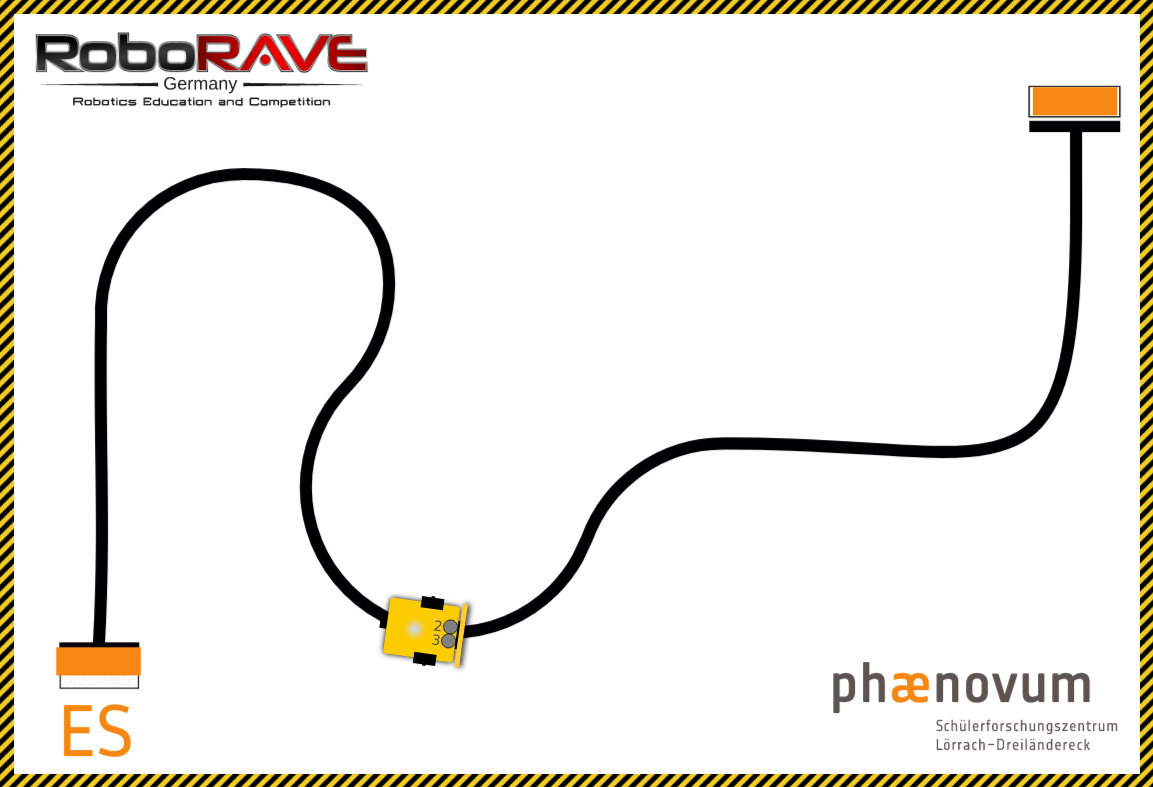
\includegraphics[width=0.3\textwidth]{images/cyberspace/linefollowing_es.png}
&
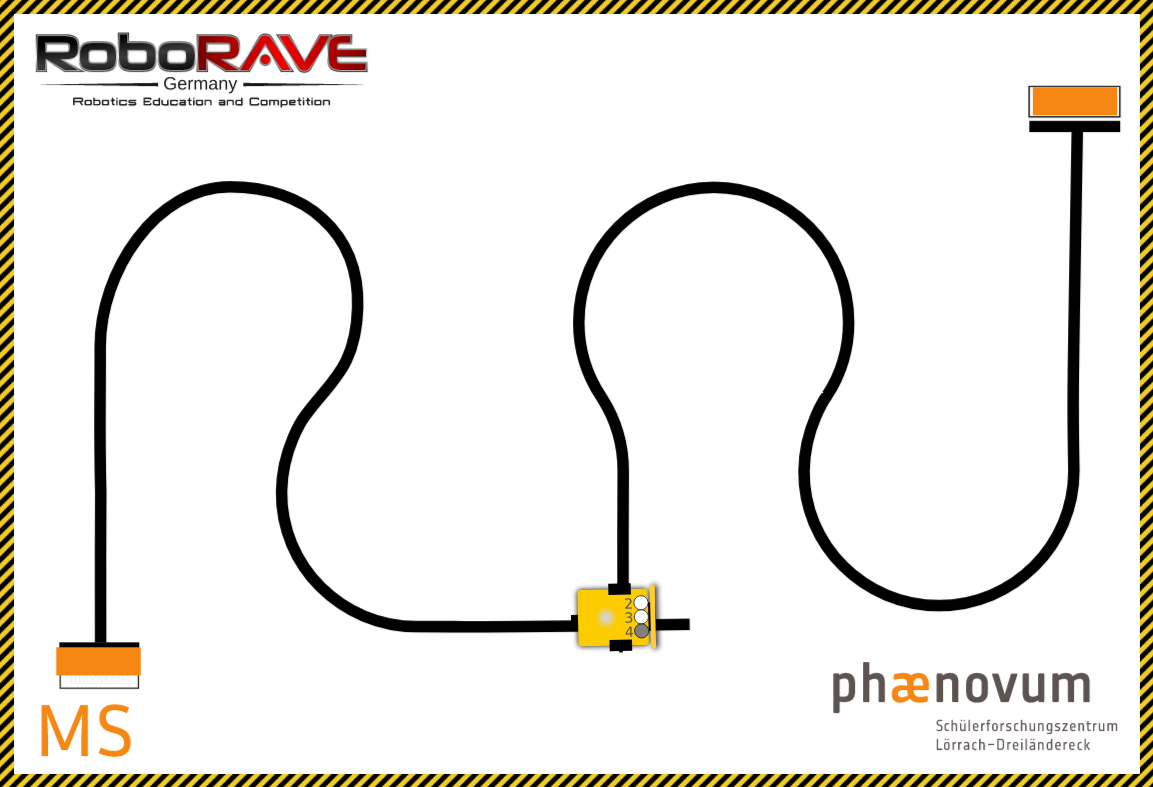
\includegraphics[width=0.3\textwidth]{images/cyberspace/linefollowing_ms.png}
&
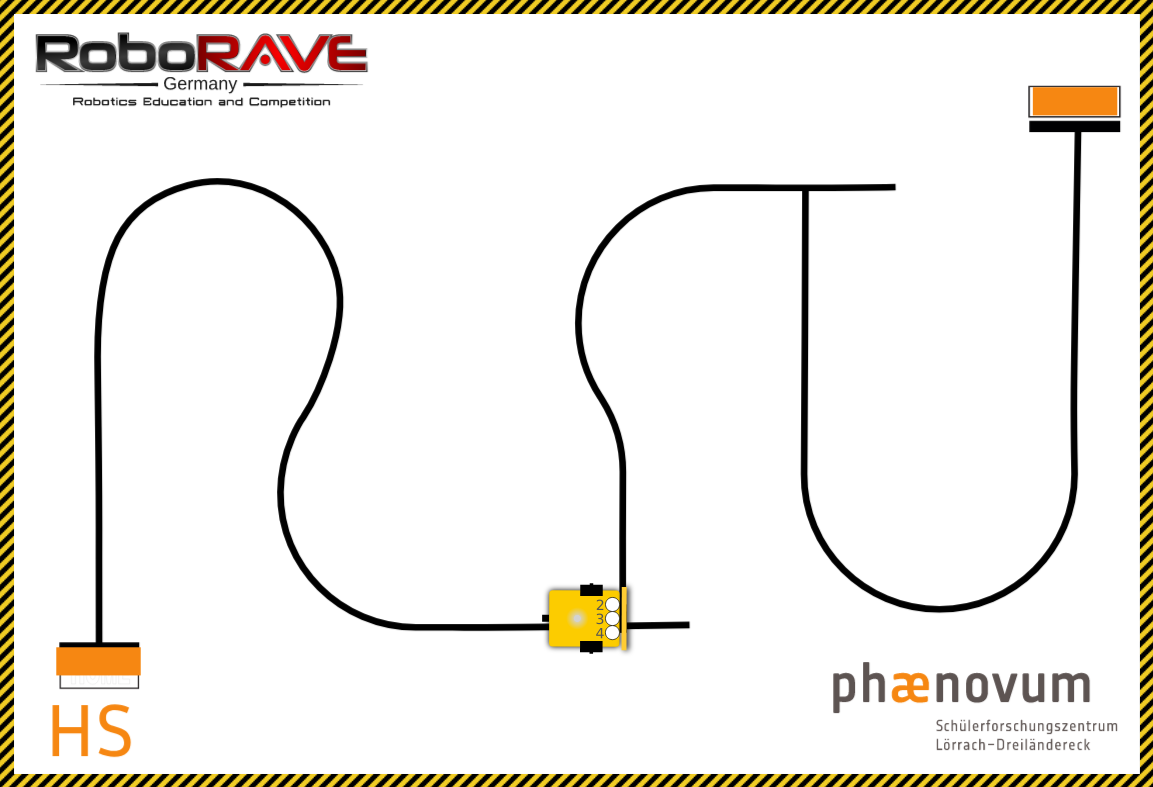
\includegraphics[width=0.3\textwidth]{images/cyberspace/linefollowing_hs.png}
\\
    		\hline
	\end{tabular}
\caption{\label{tab:table-name}Spielplan Beispiele.}
\end{table}
\end{center}


\emph{Die abgebildeten Spielpläne sind \textbf{Beispiele}. Das Design ändert sich von Jahr zu
Jahr und wird am ersten Tag des Wettbewerbes veröffentlicht.}

\subsection{Punkte}

Punkte entsprechend der Punktetabelle zuzüglich Restzeit in Sekunden.
\begin{center}
	\begin{tabular}{|c|c|c|c|c|c|} \hline
		\multirow{3}*{} & Verlässt & Passiert erste & Passiert zweite & Stoppt vor dem \\
		& Startpunkt & Abzweigung & Abzweigung & Turm \\ \hline
		ES & 50 & k.A & k.A & 100 \\ \hline
		MS & 25 & 25 & k.A & 100 \\ \hline
		HS & 25 & 25 & 25 & 50 \\ \hline
	\end{tabular}
	\begin{tabular}{|c|c|c|c|c|c|} \hline
		\multirow{3}*{} & Startet den & Passiert erste & Passiert zweite & Kommt am & Gesamt \\
		& Rückweg & Abzweigung & Abzweigung & Startpunkt an &  \\ \hline
		ES & 50 & k.A. & k.A. & 100 & 400 \\ \hline
		MS & 25 & 25 & k.A. & 100 & 400 \\ \hline
		HS & 25 & 25 & 25 & 100 & 400 \\ \hline
	\end{tabular}
\end{center}

\section{Labyrinth Challenge}

\subsection{Ziel}

Konfiguriere und programmiere einen Roboter, der (in drei Minuten) mittels
Sensoren (nicht ausschließlich mittels Drehsensoren der Motoren) den Weg
durch ein Labyrinth aus Hindernissen bis zum Ziel finden kann.

\subsection{Der Spielplan}

\begin{itemize}
	\item Spielpläne zum üben stehen unter
\href{https://cyberspace.roborave.de}{cyberspace.roborave.de} bereit
	\item Altersgruppe ES – Keine Sackgasse
	\item Altersgruppe MS – Eine Sackgasse
	\item Altersgruppen HS – Zwei Sackgassen
	\item Jedes Jahr wird ein neues Design erstellt
	\item Die Gänge des Labyrinths sind mindestens 20 cm breit
	\item Die Ecken des Labyrinths sind stets rechtwinkling, die Wände sind
		stets horizontal oder vertikal.
	\item Das Ziel ist durch ein quadratisches, farbig hervorgehobenes
		Hindernis markiert.
	\item Werbung oder gedruckte Anweisungen können überall
		auf dem Spielplan platziert sein.
\end{itemize}

\begin{center}
\begin{table}
	\begin{tabular}{|c|c|c|} \hline
		ES & MS & HS \\
		\hline
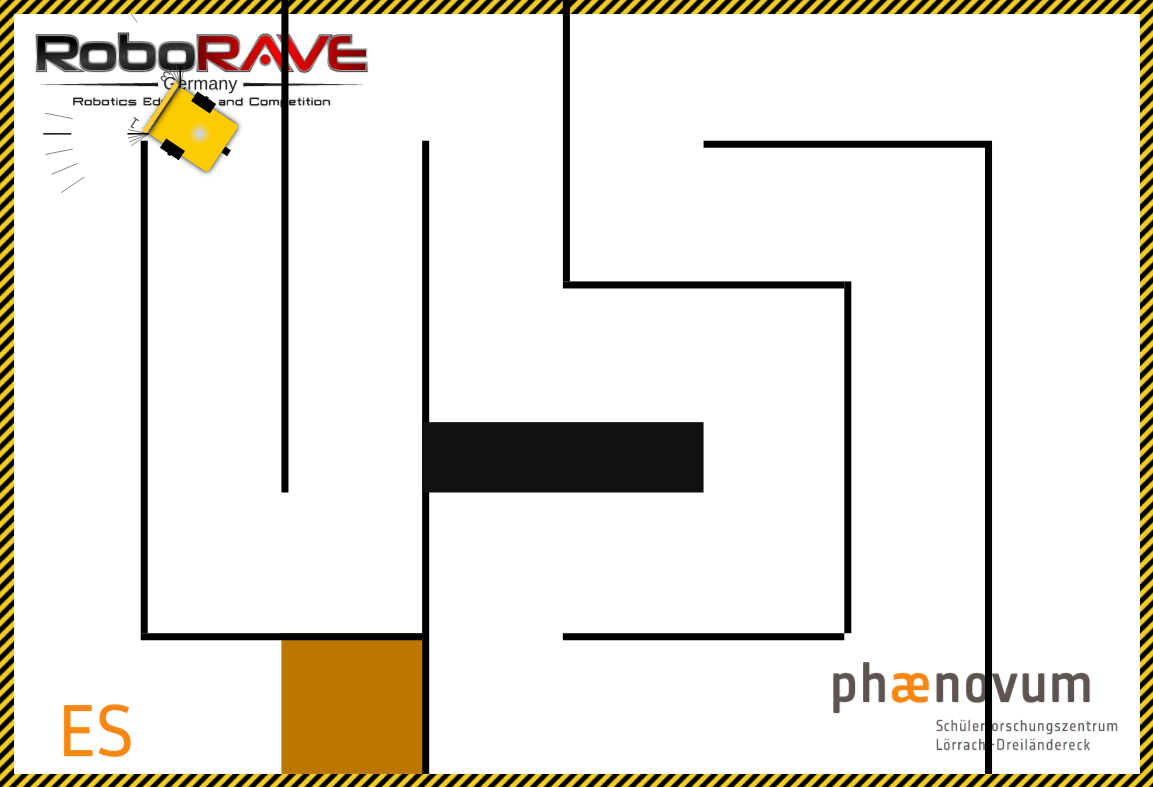
\includegraphics[width=0.3\textwidth]{images/cyberspace/labyrinth_es.png}
&
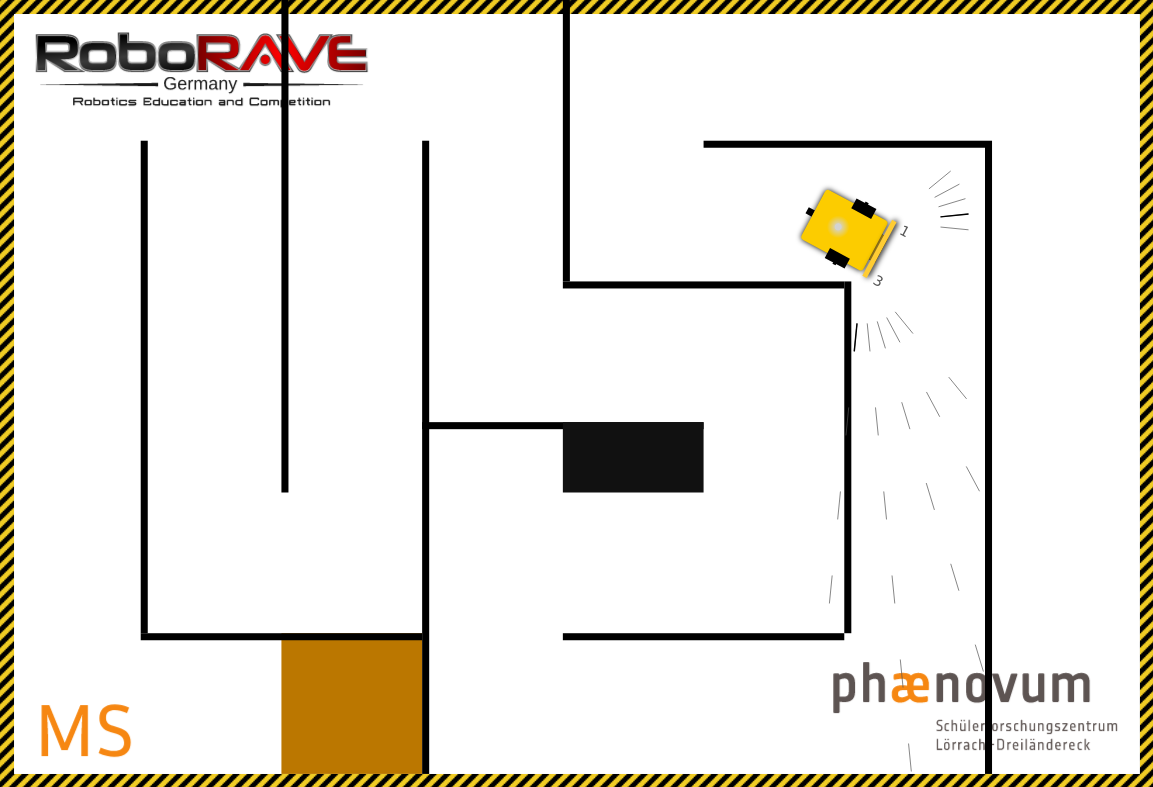
\includegraphics[width=0.3\textwidth]{images/cyberspace/labyrinth_ms.png}
&
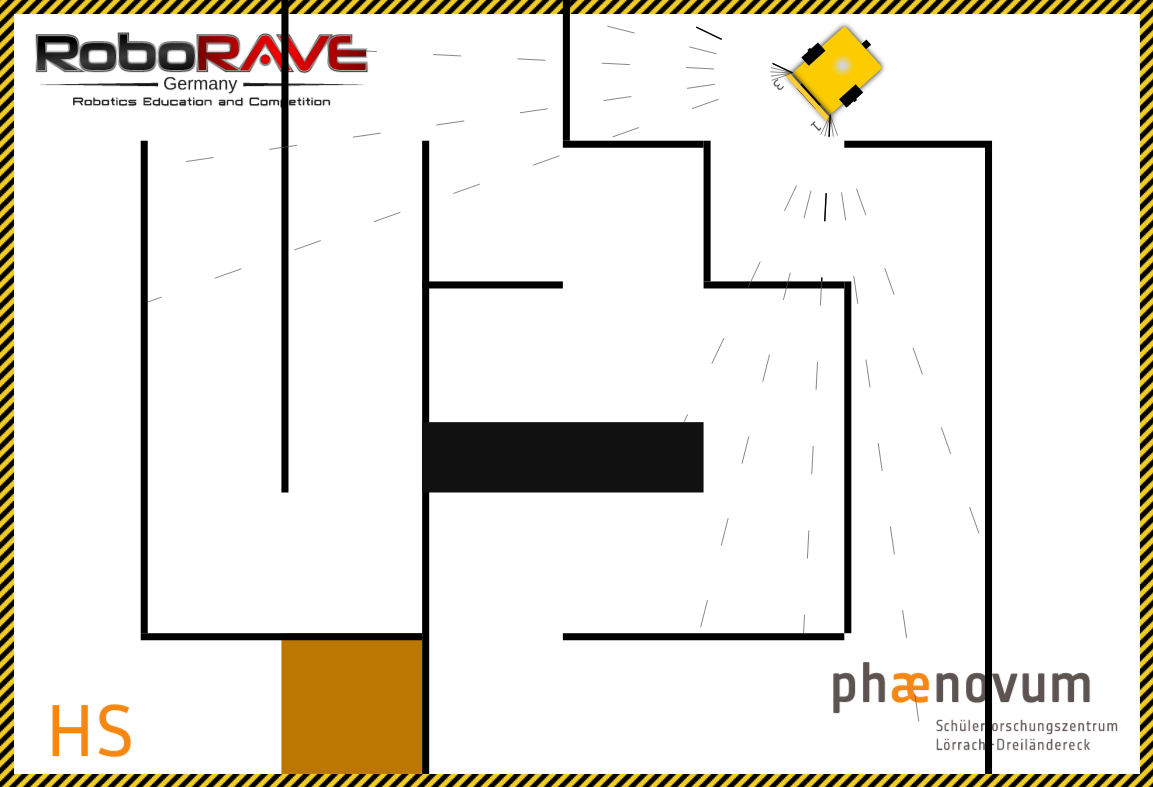
\includegraphics[width=0.3\textwidth]{images/cyberspace/labyrinth_hs.png}
\\
    		\hline
	\end{tabular}
\caption{\label{tab:table-name}Spielplan Beispiele.}
\end{table}
\end{center}

\emph{Die abgebildeten Spielpläne sind \textbf{Beispiele}. Das Design ändert sich von Jahr zu
Jahr und wird am ersten Tag des Wettbewerbes veröffentlicht.}

\subsection{Punkte}

10 Punkte pro zurückgelegtem Gang zuzüglich Restzeit in Sekunden.
Ein Gang wird durch Start, Ecke(n) oder Ziel begrenzt.

\section{Rainbow Challenge}

\subsection{Ziel}

Konfiguriere und programmiere einen Roboter, der (in fünf Minuten) mittels
Sensoren die bunten Pfade detektiert und diese in der Reihenfolge der Farben
des Regenbogens jeweils bis zum Hindernis und zurück abfährt.

\subsection{Der Spielplan}

\begin{itemize}
	\item Spielpläne zum üben stehen unter
\href{https://cyberspace.roborave.de}{cyberspace.roborave.de} bereit
	\item Jeder Pfad hat eine andere Farbe.
	\item Altersgruppe ES – 4 Pfade, Farbe und Form der Pfade ändert sich
	nicht.
	\item Altersgruppe MS – 4 Pfade, Form der Pfade ändert sich nicht,
	ihre Farbe ist zufällig.
	\item Altersgruppen HS – 6 Pfade, Form der Pfade ändert sich nicht,
	ihre Farbe ist zufällig.
	\item Farbcodes:
\begin{center}
	\begin{tabular}{|c|c|c|c|c|} \hline
		Farbe & RGB (Hexadezimal) & Rot & Grün & Blau \\ \hline
    		Rot & e40303 & 228 & 3 & 3 \\
    		Orange & ff8c00 & 255 & 140 & 0 \\
    		Gelb & ffed00 & 255 & 237 & 0 \\
    		Grün & 008026 & 0 & 128 & 38 \\
    		Blau & 004dff & 0 & 77 & 255 \\
    		Lila & 750787 & 117 & 7 & 135 \\ \hline
	\end{tabular}
\end{center}
	\item Altersgruppe ES/MS – die Pfade können die Farben rot, gelb, grün
		und blau annehmen. Das sind 24 Kombinationsmöglichkeiten.
	\item Altersgruppe HS – die Pfade können zusätzlich die Farben orange
		und lila annehmen. Das sind 720 Kombinationsmöglichkeiten.
	\item Der Mittelkreis ist von einem Rand umgeben, der vom Roboter als
		grau erkannt wird und sich von den Farben der Pfade
		unterscheidet.
	\item Altersgruppe ES/MS - der Mittelkreis ist schwarz gefüllt
	\item Altersgruppe HS - der Mittelkreis ist weiß gefüllt
	\item Der Hintergrund des Spielplans enthält keine Farben der Pfade.
	\item Altersgruppe ES/MS - der Hintergrund des Spielplans wird vom
		Farbsensor als grau erkannt.
	\item Altersgruppe HS - der Hintergrund des Spielplans wird vom
		Farbsensor als schwarz mit grauem Muster erkannt.
	\item Das Ende der Pfade ist durch ein rechteckiges, farbig
		hervorgehobenes Hindernis markiert.
	\item Altersgruppe ES/MS - die Pfade sind ca. 10 cm breit
	\item Altersgruppe HS - die Pfade sind ca. 5 cm breit
	\item Altersgruppe ES/MS - die Ecken der Pfade sind stets
		rechtwinkling, die Pfade verlaufen stets horizontal oder
		vertikal.
	\item Altersgruppe HS - die Ecken der Pfade können beliebige Winkel
		aufweisen.
	\item Werbung oder gedruckte Anweisungen können überall auf dem
		Spielplan platziert sein, jedoch nicht hinter den Pfaden.
	\item Jedes Jahr wird ein neues Design erstellt
\end{itemize}

\begin{center}
\begin{table}
	\begin{tabular}{|c|c|c|} \hline
		ES & MS & HS \\
		\hline
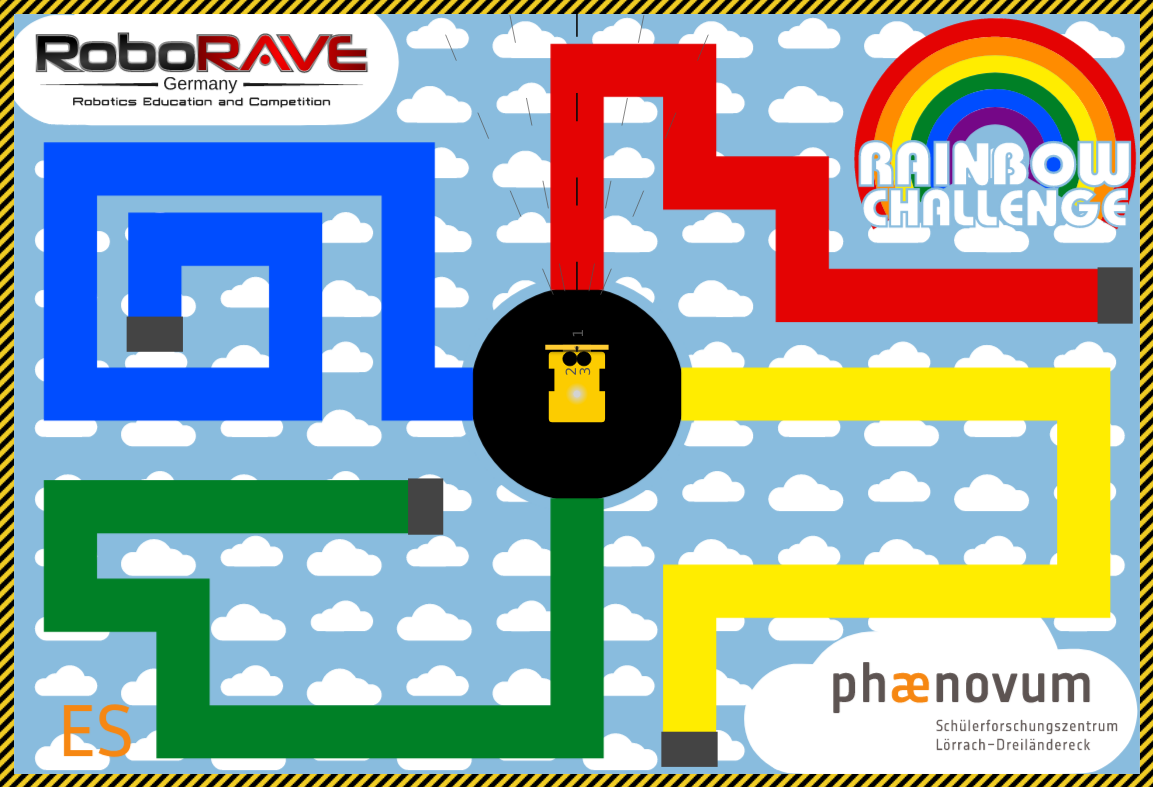
\includegraphics[width=0.3\textwidth]{images/cyberspace/rainbow_es.png}
&
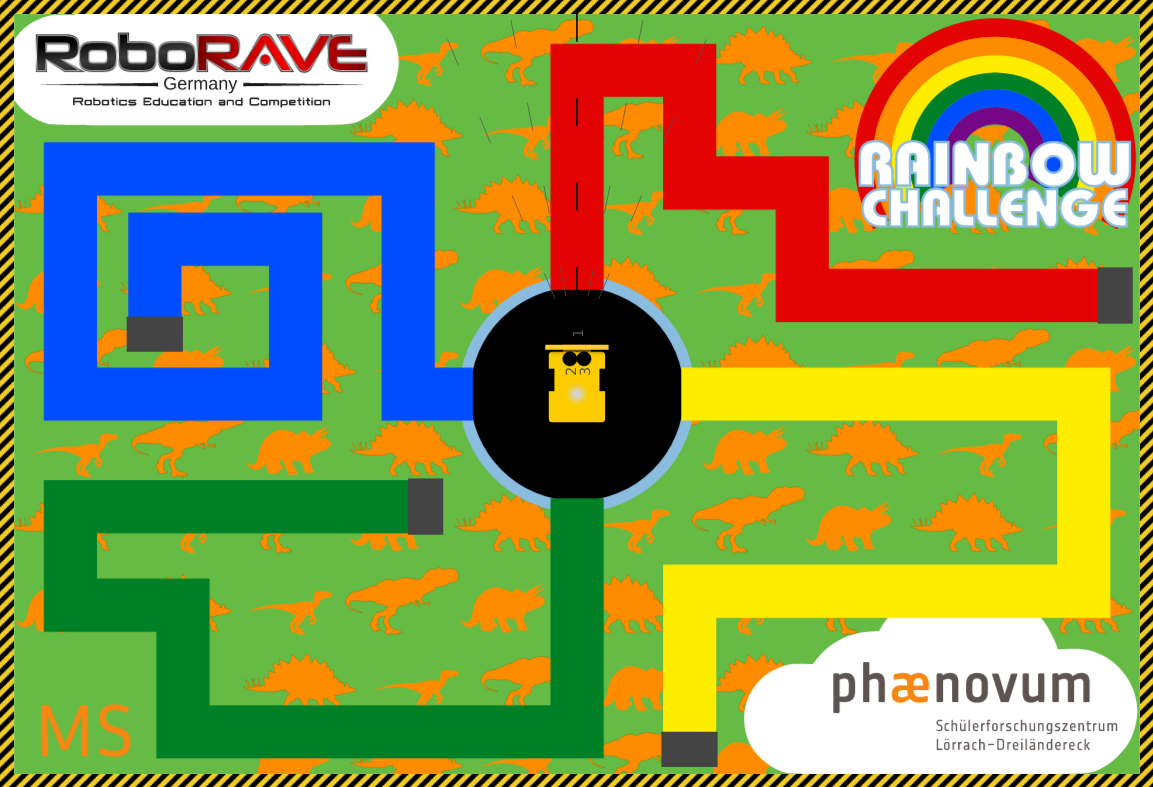
\includegraphics[width=0.3\textwidth]{images/cyberspace/rainbow_ms.png}
&
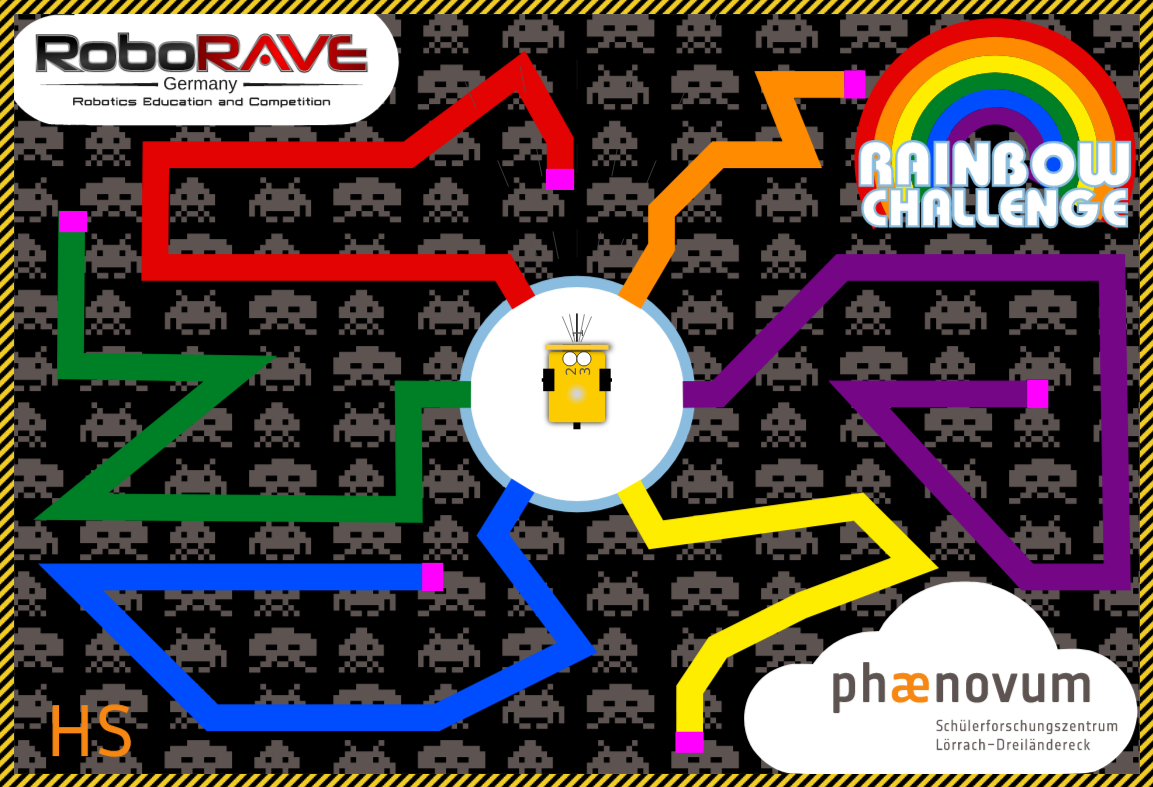
\includegraphics[width=0.3\textwidth]{images/cyberspace/rainbow_hs.png}
\\
    		\hline
	\end{tabular}
\caption{\label{tab:table-name}Spielplan Beispiele.}
\end{table}
\end{center}

\subsection{Punkte}

Für jeden Start vom richtigen Pfad 10 Punkte, 10 weitere Punkte für die Fahrt
bis zum Ende Pfades und nochmal 10 Punkte für die Rückfahrt bis zum
Mittelkreis, zuzüglich Restzeit in Sekunden.

\end{document}
